% !TeX program = lualatex
% !BIB program = biber
% Lualatex is important to render TTF fonts; with pdflatex it's just the regular one
% ratio 16:9 -- https://tex.stackexchange.com/questions/14336/

% compile two versions, inspired by https://tex.stackexchange.com/a/1501
% use the script "compile-pdf.sh"
\newif\ifhandout
% if flags.tex does not exist, create an empty file to be able to compile in TeXstudio
\input{flags}

\ifhandout
\documentclass[12pt,aspectratio=169,handout]{beamer}
\else
\documentclass[12pt,aspectratio=169]{beamer}
\fi



% TODO change "leftfootertext" to your liking
\newcommand{\leftfootertext}{Neural LMs and learning word embeddings}  % just the \title{} text by default
%\newcommand{\leftfootertext}{AI is all you need | Dr.\ Maria Mustermann}  % Your name, for instance


% ------- RUB specifics ----------
% adjust for 16:9
% https://tex.stackexchange.com/questions/354022/modifying-the-margins-of-all-slides-in-beamer
\setbeamersize{text margin left=0.3cm,text margin right=4.5cm} 


% use Metropolis as the basis theme
\usetheme[subsectionpage=progressbar]{metropolis}
% blocks with background globally
\metroset{block=fill}


\usepackage{fontspec}
% RUB fonts need to be installed
% 'UprightFont = * Light' makes sure that the base font is RubFlama Light, which looks
% lighter than RubFlama Regular (would be too thick for slides)
\setsansfont[Scale=MatchLowercase, UprightFont = * Light, BoldFont = * Bold]{RubFlama}
%\setsansfont{Arial} % Open source alternative if you don't have RubFlama

% RUB color scheme
% Dark blue: 0; 53; 96; #003560
\definecolor{RUBDarkBlue}{RGB}{0, 53, 96}

% Light yellow (table fill, etc.); 238; 250; 196; #EEFAC4
\definecolor{RUBLightYellow}{RGB}{238, 250, 196}

%Light green: 141; 174; 16
\definecolor{RUBLightGreen}{RGB}{141, 174, 16}


\setbeamercolor{titlelike}{fg=RUBDarkBlue}
\setbeamercolor{subtitle}{fg=RUBLightGreen}
\setbeamercolor{separation line}{fg=RUBLightGreen}
\setbeamercolor{frametitle}{bg=white, fg=RUBDarkBlue}

% horizontal line on title page and sections
\setbeamercolor{alerted text}{fg=RUBLightGreen}


% Adjust footer bottom (too large by default)
\setbeamertemplate{footline}{%
  \begin{beamercolorbox}[wd=\textwidth, sep=2ex]{footline}%
    \usebeamerfont{page number in head/foot}%
    \usebeamertemplate*{frame footer}
    \hfill%
    \usebeamertemplate*{frame numbering}
  \end{beamercolorbox}%
}


% Lab name, numbering, etc. in footer
\setbeamertemplate{frame numbering}{TrustHLT --- Prof.\ Dr.\ Ivan Habernal \hspace*{1ex} \includegraphics[width=7em]{img/rub-logo.pdf}\hspace*{1ex}}

\setbeamertemplate{frame footer}{\hspace*{1ex}\insertframenumber \hspace*{2ex} \leftfootertext}

% adjust the background to be completely white
\setbeamercolor{background canvas}{bg=white}

% logos on the title page
\titlegraphic{%
	\begin{picture}(0,0)
		\put(435,0){\makebox(0,0)[rt]{\includegraphics[width=7em]{img/rub-logo.pdf}}}
		\put(435,-170){\makebox(0,0)[rt]{\includegraphics[width=4em]{img/logo-trusthlt.pdf}}}
		\put(435,-196){\makebox(0,0)[rt]{\includegraphics[width=9em]{img/logo-rctrust.pdf}}}
	\end{picture}%
}


% show TOC at every section start
\AtBeginSection{
	\frame{
		\vspace{2em}
		\sectionpage
		\hspace*{2.2em}\begin{minipage}{10cm}
			\tableofcontents[currentsection]
		\end{minipage}
	}
}

% TOC without subsection
\setcounter{tocdepth}{1} % only-- part,chapters,sections 

% bullet points: rectangles
\useinnertheme{rectangles}
\setbeamercolor{itemize item}{fg=RUBLightGreen}
\setbeamercolor{itemize subitem}{fg=RUBLightGreen}
% enumerate: blue background for better readability
\setbeamercolor{item projected}{bg=RUBDarkBlue}

% make boxes (example, block, etc.) background lighter for readability
\setbeamercolor{block title}{%
	use=normal text,
	fg=normal text.fg,
	bg=normal text.bg!90!fg % lighter background in block title
}
\setbeamercolor{block body}{
	use={block title, normal text},
	bg=block title.bg!30!normal text.bg % lighter background in block body
}


% RUB colors in blocks
\setbeamercolor{block title alerted}{%
	use={block title, alerted text},
	bg=RUBDarkBlue,
	%fg=RUBLightYellow % looks bad
	fg=white % better contrast
}

\setbeamercolor{block title example}{%
	use={block title, example text},
	fg=RUBLightGreen
}


% ------- end of RUB specifics ----------

% all itemize with pause by default
%\beamerdefaultoverlayspecification{<+->}


% typeset mathematics on serif
\usefonttheme[onlymath]{serif}

% better bibliography using biber as backend
\usepackage[natbib=true,backend=biber,style=authoryear-icomp,maxbibnames=30,maxcitenames=9,uniquelist=false,giveninits=true,doi=false,url=false,dashed=false,isbn=false]{biblatex}
% shared bibliography
\addbibresource{../../nlpwdl-bibliography.bib}
% disable "ibid" for repeated citations
\boolfalse{citetracker}



\usepackage{xspace}


% for derivatives, https://tex.stackexchange.com/a/412442
\usepackage{physics}

\usepackage{tikz}
\usetikzlibrary{matrix, positioning}
\usetikzlibrary{angles,quotes} % for angles
\usetikzlibrary{backgrounds} % background
\usetikzlibrary{decorations.pathreplacing} % curly braces
\usetikzlibrary{calligraphy}
\usetikzlibrary{calc} % for neural nets

% for plotting functions
\usepackage{pgfplots}
\usepgfplotslibrary{dateplot}

% sub-figures
\usepackage{caption}
\usepackage{subcaption}

% book tabs
\usepackage{booktabs}


% argmin, argmax
\usepackage{amsmath}
\DeclareMathOperator*{\argmax}{arg\!\max}
\DeclareMathOperator*{\argmin}{arg\!\min}
% softmax
\DeclareMathOperator*{\softmax}{soft\!\max}
% Mask
\DeclareMathOperator*{\mask}{mask}

% bold math
\usepackage{bm}

% for \mathclap
\usepackage{mathtools}

% algorithms
\usepackage[noend]{algpseudocode}


% for neurons and layers in tikz
\tikzset{
	neuron/.style={draw, rectangle, inner sep=2pt, minimum width=0.75cm, fill=blue!20},
	param/.style={draw, rectangle, inner sep=2pt, minimum width=0.75cm, fill=green!20},
	constant/.style={draw, rectangle, inner sep=2pt, minimum width=0.75cm, fill=black!15},
	% for citation nodes right top
	ref/.style={anchor = north east, text width=7.8cm, yshift=-1.3cm, xshift=-0.2cm, scale=0.5},
	state/.style={rectangle, inner sep=2pt, minimum width=0.75cm, fill=black!5},
}

% added in lecture 10
\tikzset{
	mtx/.style={
		matrix of math nodes,
		left delimiter={[}, right delimiter={]}
	},
	hlt/.style={opacity=0.1, line width=4 mm, line cap=round},
	hltr/.style={opacity=0.5, rounded corners=2pt, inner sep=-1pt}
}

% for strike-through text (added in Lecture 06)
\usepackage[normalem]{ulem}

% added in Lecture 7
% RNN
\DeclareMathOperator*{\rnn}{RNN}
% RNN star
\DeclareMathOperator*{\rnnstar}{RNN^{*}}
% bi-RNN
\DeclareMathOperator*{\birnn}{biRNN}


% added in Lecture 9
\usetikzlibrary{fit} % for hightligting by calling "fit"

% algorithms
\usepackage[noend]{algpseudocode}



\title{Natural Language Processing with Deep Learning}
\subtitle{Lecture 6 --- Neural language models and learning word embeddings}
\date{November 28, 2024}
\author{Prof.\ Dr.\ Ivan Habernal}
\institute{
\texttt{www.trusthlt.org} \\
Trustworthy Human Language Technologies Group (TrustHLT) \\
Ruhr University Bochum \& Research Center Trustworthy Data Science and Security}


\begin{document}

\maketitle



\section{Language modeling}


\begin{frame}{Recap: What was the task of a language model again?}

\begin{block}{LM as a conditional probability predictor}
Given a sequence of $k$ words, return a probability distribution over $V$ (the vocabulary) for the next possible word
\end{block}

In detail, compute
$$
\Pr(W_{\text{next}} = v \mid W_1, W_2, \ldots, W_k)
$$
for all possible words $v$ from vocabulary $V$

\end{frame}



\begin{frame}{Example}

\emph{So I was at this party at Joe's place last night, but man I was so tired, so like at about midnight I said, Joe, I'm \_\_}

$\Pr(W_{\text{next}} = v \mid W_1 = \text{`So'}, W_2 = \text{`I'}, \ldots)$

\medskip

\begin{columns}[t]
\begin{column}{0.5\linewidth}
Higher $\Pr$:
\begin{itemize}
\item leaving
\item out
\item calling \emph{(it a night)}
\item gonna \emph{(head home)}
\item $\ldots$
\end{itemize}
\end{column}
\begin{column}{0.5\linewidth}
Lower $\Pr$:
\begin{itemize}
\item hungry
\item in \emph{(love)}
\item $\ldots$
\end{itemize}
\end{column}

\end{columns}

\end{frame}



\begin{frame}{LM looks like... a text classification task!}

\begin{block}{Text classification}
Given a text (we know how to turn in into a feature vector), predict \textbf{its label} from a set of arbitrarily ordered categories (\textbf{e.g., \{neg, neu, pos\}}). We typically predict probability for each \textbf{label} by using softmax over the \textbf{categories}.
\end{block}
\pause

\begin{block}{LM}
Given a text (we know how to turn in into a feature vector), predict \textbf{the next word} from a set of arbitrarily ordered categories (\textbf{the vocabulary}). We typically predict probability for each \textbf{word} by using softmax over the \textbf{vocabulary}.
\end{block}

\end{frame}



\subsection{Neural language models}

\begin{frame}{Neural LMs}

\begin{block}{LM as `text classification' again}
Given a text (we know how to turn in into a feature vector), predict \textbf{the next word} from a set of arbitrarily ordered categories (\textbf{the vocabulary}). We typically predict probability for each \textbf{word} by using softmax over the \textbf{vocabulary}.
\end{block}
	
Let's build a neural network to solve this task
\pause
	\begin{itemize}
		\item Input: a $k$-gram of words $w_{1:k}$
		\item Desired output: a probability distribution over the vocabulary $V$ for the next word $w_{k+1}$
	\end{itemize}
	
\end{frame}

\begin{frame}{Embedding layer}
	
	If the input are symbolic \textbf{categorical features}
	\begin{itemize}
		\item e.g., words from a closed vocabulary
	\end{itemize}
	it is common to associate each possible feature value
	\begin{itemize}
		\item i.e., each word in the vocabulary
	\end{itemize}
	with a $d$-dimensional vector for some $d$
	
	\bigskip
	
	These vectors are also \emph{parameters} of the model, and are trained jointly with the other parameters
	
\end{frame}

\begin{frame}{Embedding layer: Lookup operation}
	
	Mapping from a symbolic feature such as \texttt{word-number-48} to $d$-dimensional vectors is performed by an embedding layer (a lookup layer)
	
	The parameters in an embedding layer is a matrix $\bm{E}^{\abs{V} \times d}$, each row corresponds to a different word in the vocabulary
	
	The lookup operation is then indexing $v(w)$, e.g.,
	$$v(w) = v_{48} = \bm{E}_{[48,:]}$$
	
	If the symbolic feature is a one-hot vector $\bm{x}$, the lookup operation can be implemented as the multiplication $\bm{x} \bm{E}$
	
\end{frame}


\begin{frame}{Network concatenating 3 words as embeddings ($d_w = 50$)}
	\vspace{-1em}
	%	$$	f(\bm{x}) = g \left(	\bm{x} \bm{W^1} + \bm{b^1}	\right)	\bm{W^2} + \bm{b^2}	$$
	\begin{figure}
		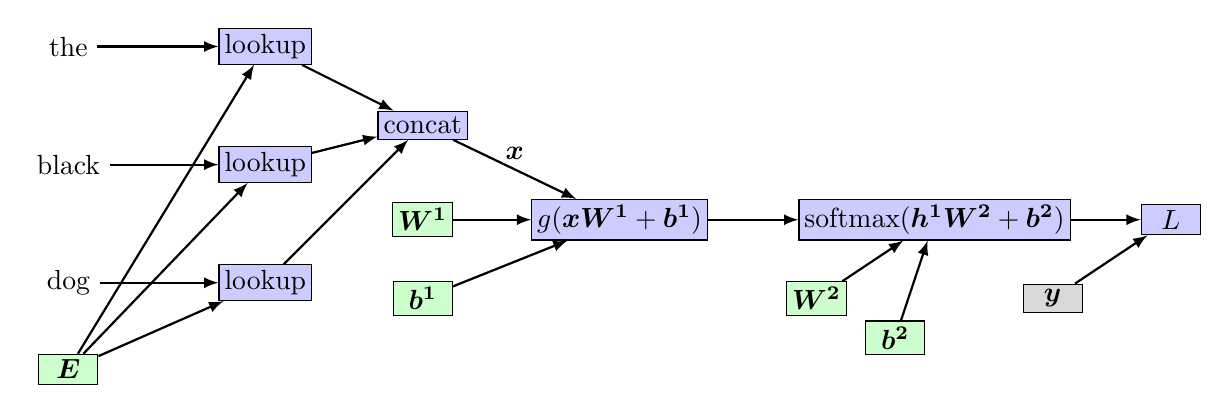
\begin{tikzpicture}	
			%\node (a1) [draw, circle, inner sep=0pt, minimum width=0.75cm, fill=green!20] {$a_1$};
			
			\node (the) {the};
			\node (black) [below of=the, yshift=-0.5cm]{black};
			\node (dog) [below of=black, yshift=-0.5cm]{dog};
			\node (e) [param, below of=dog, yshift=-0.1cm] {$\bm{E}$};
			
			\node (lookup1) [neuron, right of=the, xshift=1.5cm] {lookup};
			\node (lookup2) [neuron, below of=lookup1, yshift=-0.5cm] {lookup};
			\node (lookup3) [neuron, below of=lookup2, yshift=-0.5cm] {lookup};			
			\node (concat) [neuron, right of=lookup1, xshift=1cm, yshift=-1cm] {concat};
			
			
			%			\node (x) [constant, right of=concat, xshift=1cm] {$\bm{x}$};
			\node (w) [param, below of=concat, yshift=-0.2cm] {$\bm{W^1}$};
			\node (b) [param, below of=w] {$\bm{b^1}$};
			
			\node (f1) [neuron, right of=w, xshift=1.5cm] {$g(\bm{x} \bm{W^1} + \bm{b^1})$};
			
			\node (f2) [neuron, right of=f1, xshift=3cm] {$\softmax(\bm{h^1} \bm{W^2} + \bm{b^2})$};
			
			\node (w2) [param, below of=f2, xshift=-1.5cm, yshift=0cm] {$\bm{W^2}$};
			\node (b2) [param, below of=f2, xshift=-0.5cm, yshift=-0.5cm] {$\bm{b^2}$};
			
			\node (l) [neuron, right of=f2, xshift=2cm] {$L$};
			\node (y) [constant, below of=f2, xshift=1.5cm] {$\bm{y}$};
			
			\begin{scope}[thick, black, ->, >=latex]
				\draw (the) -- (lookup1);
				\draw (black) -- (lookup2);
				\draw (dog) -- (lookup3);
				\draw (e) -- (lookup1);
				\draw (e) -- (lookup2);
				\draw (e) -- (lookup3);
				
				\draw (lookup1) -- (concat);
				\draw (lookup2) -- (concat);
				\draw (lookup3) -- (concat);								
				
				\draw (concat) -- (f1) node [midway, above] {$\bm{x}$};
				\draw (w) -- (f1);
				\draw (b) -- (f1);
				\draw (f1) -- (f2);
				\draw (f2) -- (l);
				\draw (w2) -- (f2);
				\draw (b2) -- (f2);
				\draw (y) -- (l);
			\end{scope}	
		\end{tikzpicture}
	\end{figure}	
	
	Each word $\in \mathbb{R}^{\abs{V}}$ (one hot), 
	$\bm{E} \in \mathbb{R}^{\abs{V} \times 50}$, each lookup output $\in \mathbb{R}^{50}$, concat output $\bm{x} \in \mathbb{R}^{150}$
	
	
\end{frame}



\begin{frame}{Simplify notation: Lookup as $v$, linear layer with params}
	\vspace{-1em}
	%	$$	f(\bm{x}) = g \left(	\bm{x} \bm{W^1} + \bm{b^1}	\right)	\bm{W^2} + \bm{b^2}	$$
	\begin{figure}
		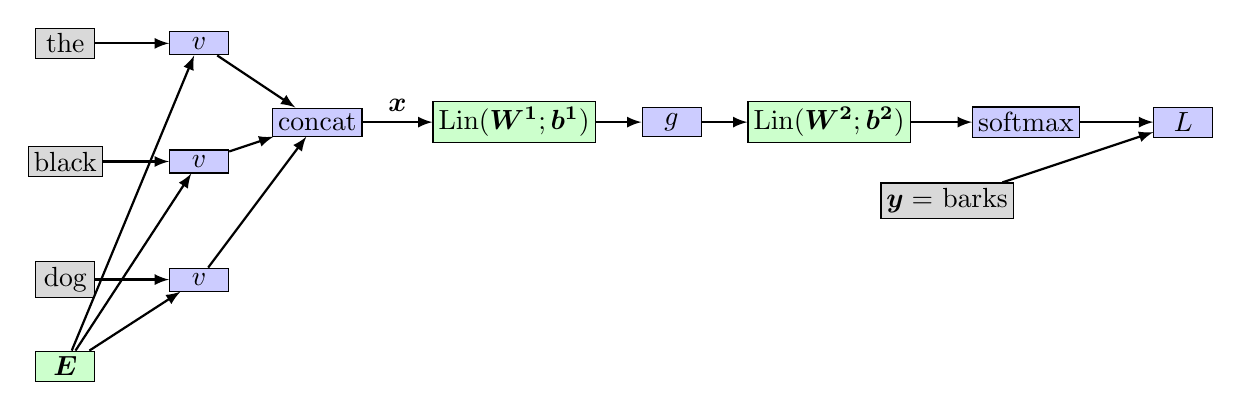
\begin{tikzpicture}	
			%\node (a1) [draw, circle, inner sep=0pt, minimum width=0.75cm, fill=green!20] {$a_1$};
			
			\node (the) [constant] {the};
			\node (black) [constant, below of=the, yshift=-0.5cm]{black};
			\node (dog) [constant, below of=black, yshift=-0.5cm]{dog};
			\node (e) [param, below of=dog, yshift=-0.1cm] {$\bm{E}$};
			
			\node (lookup1) [neuron, right of=the, xshift=0.7cm] {$v$};
			\node (lookup2) [neuron, below of=lookup1, yshift=-0.5cm] {$v$};
			\node (lookup3) [neuron, below of=lookup2, yshift=-0.5cm] {$v$};			
			\node (concat) [neuron, right of=lookup1, xshift=0.5cm, yshift=-1cm] {concat};
			
			
			%			\node (x) [constant, right of=concat, xshift=1cm] {$\bm{x}$};
			\node (f1) [param, right of=concat, xshift=1.5cm] {Lin$(\bm{W^1};\bm{b^1})$};
			
			\node (g) [neuron, right of=f1, xshift=1cm] {$g$};
			\node (f2) [param, right of=g, xshift=1cm] {Lin$(\bm{W^2};\bm{b^2})$};
			
			\node (softmax) [neuron, right of=f2, xshift=1.5cm] {$\softmax$};
			
			\node (l) [neuron, right of=softmax, xshift=1cm] {$L$};
			\node (y) [constant, below of=f2, xshift=1.5cm] {$\bm{y} =$ barks};
			
			\begin{scope}[thick, black, ->, >=latex]
				\draw (the) -- (lookup1);
				\draw (black) -- (lookup2);
				\draw (dog) -- (lookup3);
				\draw (e) -- (lookup1);
				\draw (e) -- (lookup2);
				\draw (e) -- (lookup3);
				
				\draw (lookup1) -- (concat);
				\draw (lookup2) -- (concat);
				\draw (lookup3) -- (concat);								
				
				\draw (concat) -- (f1) node [midway, above] {$\bm{x}$};
				\draw (f1) -- (g);
				\draw (g) -- (f2);
				\draw (f2) -- (softmax);
				\draw (softmax) -- (l);
				\draw (y) -- (l);
			\end{scope}	
		\end{tikzpicture}
	\end{figure}	
	
	the, black, dog, $\bm{y}$ = one-hot encoding, $\mathbb{R}^{\abs{V}}$
	
	Loss $L$ and gold label $\bm{y}$ --- only for training
\end{frame}

\begin{frame}{Neural LMs: Input fix-sized feature vector}
	

Each input word $w_k$ is associated with an embedding vector $v(w) \in \mathbb{R}^{d_w}$ ($d_w$ --- word embedding dimensionality)

Input vector $\bm{x}$ is a concatenation of $k$ words
$$
\bm{x} = \left[ v(w_1); v(w_2); \ldots; v(w_k) \right]
$$
	
\end{frame}

\begin{frame}{Neural LMs}
	
	MLP with one (or more) hidden layers
	
	$$
	\begin{aligned}
		v(w) &= \bm{E}_{w,:} \\
		\bm{x} &= \left[ v(w_1); v(w_2); \ldots; v(w_k) \right] \\
		\bm{h} &= g(\bm{x} \bm{W^1} + \bm{b^1}) \\
		\hat{\bm{y}} = \Pr(W_i \mid w_{1:k}) &= \softmax (\bm{h} \bm{W^2} + \bm{b^2})
	\end{aligned}
	$$
	
	Output dimension: $\hat{\bm{y}} \in \mathbb{R}^{\abs{V}}$
	
\end{frame}

\begin{frame}{Training neural LMs}
	
	Where to get training examples?
	
	Training examples are simply word $k$-grams from an unlabeled corpus
	\begin{itemize}
		\item Identities of the first $k - 1$ words are used as features
		\item The last word is used as the target label for the classification
	\end{itemize}
	
	The model is trained using cross-entropy loss
\end{frame}

\begin{frame}{Some advantages of neural LMs}
	
$\approx$ linear increase in parameters with $k + 1$ (better than `classical' LMs)
	
\end{frame}

\begin{frame}{Generating text with language models}
	
	We can generate (``sample") random sentences from the model according to their probability
	
	\begin{enumerate}
		\item Predict a probability distribution over the vocabulary conditioned on the start symbol <s>
		\item Draw the first word from the predicted distribution
		\item Predict a probability distribution over the vocabulary conditioned on the start symbol and the first word
		\item Draw the second word from the predicted distribution
		\item Repeat until generated \emph{end-of-sentence} symbol </s> (or <EOS>)
	\end{enumerate}
	
	
\end{frame}

\begin{frame}{Learned word representations as a by-product}
\vspace{-1em}
\begin{figure}
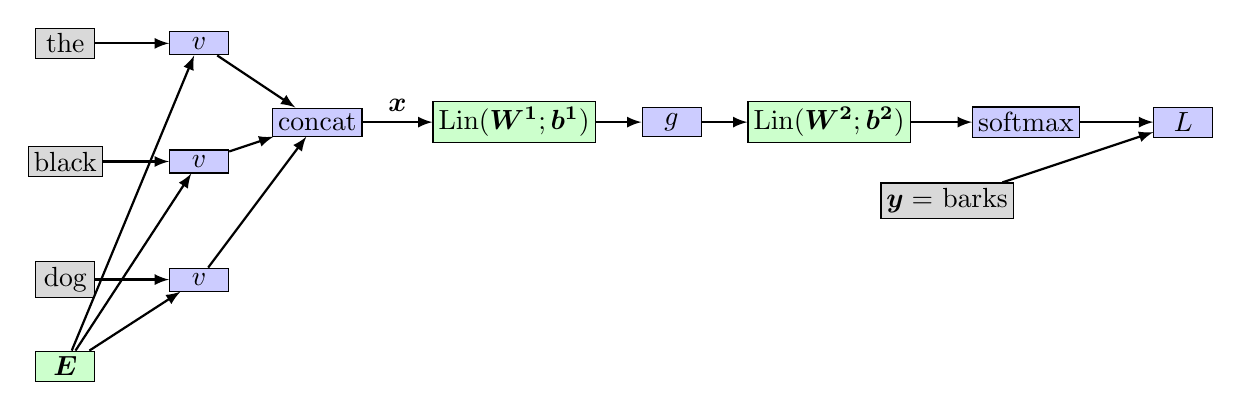
\begin{tikzpicture}	
	%\node (a1) [draw, circle, inner sep=0pt, minimum width=0.75cm, fill=green!20] {$a_1$};
	
	\node (the) [constant] {the};
	\node (black) [constant, below of=the, yshift=-0.5cm]{black};
	\node (dog) [constant, below of=black, yshift=-0.5cm]{dog};
	\node (e) [param, below of=dog, yshift=-0.1cm] {$\bm{E}$};
	
	\node (lookup1) [neuron, right of=the, xshift=0.7cm] {$v$};
	\node (lookup2) [neuron, below of=lookup1, yshift=-0.5cm] {$v$};
	\node (lookup3) [neuron, below of=lookup2, yshift=-0.5cm] {$v$};			
	\node (concat) [neuron, right of=lookup1, xshift=0.5cm, yshift=-1cm] {concat};
	
	
	%			\node (x) [constant, right of=concat, xshift=1cm] {$\bm{x}$};
	\node (f1) [param, right of=concat, xshift=1.5cm] {Lin$(\bm{W^1};\bm{b^1})$};
	
	\node (g) [neuron, right of=f1, xshift=1cm] {$g$};
	\node (f2) [param, right of=g, xshift=1cm] {Lin$(\bm{W^2};\bm{b^2})$};
	
	\node (softmax) [neuron, right of=f2, xshift=1.5cm] {$\softmax$};
	
	\node (l) [neuron, right of=softmax, xshift=1cm] {$L$};
	\node (y) [constant, below of=f2, xshift=1.5cm] {$\bm{y} =$ barks};
	
	\begin{scope}[thick, black, ->, >=latex]
		\draw (the) -- (lookup1);
		\draw (black) -- (lookup2);
		\draw (dog) -- (lookup3);
		\draw (e) -- (lookup1);
		\draw (e) -- (lookup2);
		\draw (e) -- (lookup3);
		
		\draw (lookup1) -- (concat);
		\draw (lookup2) -- (concat);
		\draw (lookup3) -- (concat);								
		
		\draw (concat) -- (f1) node [midway, above] {$\bm{x}$};
		\draw (f1) -- (g);
		\draw (g) -- (f2);
		\draw (f2) -- (softmax);
		\draw (softmax) -- (l);
		\draw (y) -- (l);
	\end{scope}	
\end{tikzpicture}
\end{figure}
	
Each row of $\bm{E}$ learns a word representation
	
	
\end{frame}

\section{Word embeddings}

\begin{frame}{Motivation}

I give you a large corpus of plain text data

Can you build a model that will answer any of the `word analogy' tasks?

\begin{itemize}
	\item `Germany to Berlin is like France to ?'
	\item `Man to king is like woman to ?'
\end{itemize}

\end{frame}



\section{We need to talk about the dot product}



\begin{frame}{Geometry of dot product}
	
	\onslide<1->{
		For two $n$-dimensional vectors $\bm{u}$ and $\bm{v}$
	}
	
	$$
	\begin{matrix}
		\onslide<2->{\text{Algebraic}} & \qquad & \onslide<3->{\text{Geometric}} \\
		\onslide<2->{\bm{u} \cdot \bm{v} = \sum_{i = 1}^{n} \bm{u}_{[i]} \bm{v}_{[i]}}
		& \qquad
		& \onslide<3->{\bm{u} \cdot \bm{v} = \norm{\bm{u}} \norm{\bm{v}} \cos (\theta)}
	\end{matrix}
	$$
	
	%	The dot product of two vectors returns a scalar. It gives us some insights into how the two vectors are related.
	
	%	Geometric formula:
	
	%		If vector u is a unit vector, the dot product is a perpendicular projection of y on vector u
	
	\begin{columns}
		
		\begin{column}{0.4\linewidth}
			
			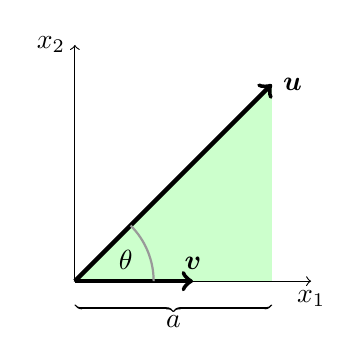
\begin{tikzpicture}
				\onslide<1->{
					\draw[->] (0,0)--(3,0) node[below]{$x_1$};
					\draw[->] (0,0)--(0,3) node[left]{$x_2$};
					\draw[->, ultra thick] (0,0)--(2.5,2.5) node[right]{$\bm{u}$};
					\draw[->, ultra thick] (0,0)--(1.5,0) node[right, above]{$\bm{v}$};
				}
				
				\onslide<3->{
					\draw
					(1,1) coordinate (a)
					-- (0,0) coordinate (b)
					-- (1,0) coordinate (c)
					pic["$\theta$", draw=black!40, thick, -, angle eccentricity=0.7, angle radius=1cm]
					{angle=c--b--a};
				}
				
				
				\begin{scope}[on background layer]
					\onslide<4->{
						\path [fill=green!20] (0,0) -- (2.5,2.5) -- (2.5,0) -- cycle;
					}
				\end{scope}
				\onslide<4->{	
					\draw [decorate, thick, decoration = {calligraphic brace}] (2.5,-0.3) --  (0,-0.3) node [midway, below]{$a$};
				}
				
			\end{tikzpicture}
			
		\end{column}
		
		\begin{column}{0.5\linewidth}
			
			\onslide<4->{
				Scalar projection:
				$$\implies a = \frac{\bm{u} \cdot \bm{v}}{\norm{\bm{v}}}$$
			}
			
			
		\end{column}
		
		
	\end{columns}
	
\end{frame}



\begin{frame}{Dot product of unit vectors (aka.\ cosine similarity)}
	For unit vectors $\bm{u}, \bm{v}$:
	\onslide<2->{
		$$
		\bm{u} \cdot \bm{v} = \norm{\bm{u}} \norm{\bm{v}} \cos (\theta)
		\quad \to \quad
		\bm{u} \cdot \bm{v} = \cos (\theta)
		$$
	}
	\begin{columns}
		\begin{column}{0.3\linewidth}
			%		\vspace{3em} % why the heck this works as negative space?!
			\vspace{-2em}
			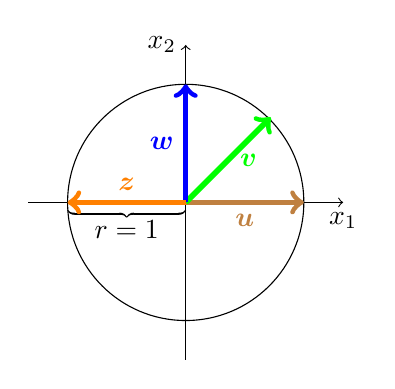
\begin{tikzpicture}
				\begin{scope}[on background layer]
					\onslide<1->{
						\draw[->] (-2,0)--(2,0) node[below]{$x_1$};
						\draw[->] (0,-2)--(0,2) node[left]{$x_2$};
						\draw (0,0) circle [radius=1.5];
						\draw [decorate, thick, decoration = {calligraphic brace}] (0,-0.1) --  (-1.5,-0.1) node [midway, below]{$r = 1$};
					}
				\end{scope}
				
				\onslide<1->{
					\draw[->, line width=2pt, brown] (0,0)--(1.5,0) node[midway, below]{$\bm{u}$};
					\draw[->, line width=2pt, green] (0,0)--(1.08,1.08) node[midway, right]{$\bm{v}$};
				}
				\onslide<4->{
					\draw[->, line width=2pt, blue] (0,0)--(0,1.5) node[midway, left]{$\bm{w}$};
				}
				\onslide<5->{
					\draw[->, line width=2pt, orange] (0,0)--(-1.5,0) node[midway, above]{$\bm{z}$};				
				}
			\end{tikzpicture}
			
		\end{column}
		\begin{column}{0.45\linewidth}
			\onslide<3->{
				\vspace{-1em}
				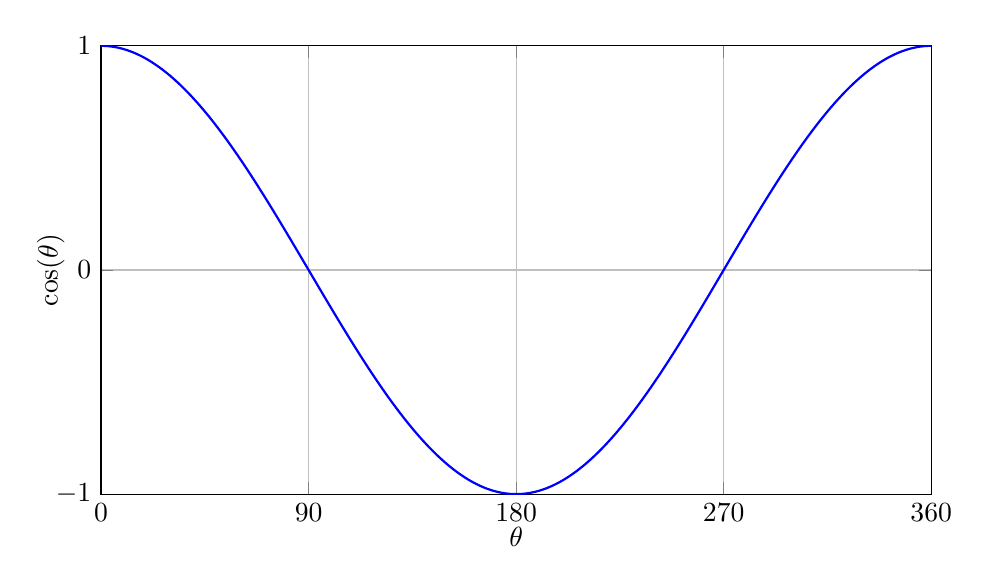
\begin{tikzpicture}
					\begin{axis}[
						xmin = 0, xmax = 360,
						ymin = -1, ymax = 1,
						xtick distance = 90,
						ytick distance = 1,
						grid = major,
						%						minor tick num = 4,
						major grid style = {lightgray},
						minor grid style = {lightgray!25},
						width = \textwidth,
						height = 0.6\textwidth,
						legend pos = north east,
						xlabel={$\theta$},
						xlabel shift=-0.5em,
						ylabel ={$\cos(\theta)$},
						ylabel shift=-1em,
						]
						
						\addplot[
						domain = 0.001:360,
						samples = 200,
						smooth,
						thick,
						blue,
						] {cos(x)};
						
					\end{axis}			
				\end{tikzpicture}
			}
			\vspace{-1em}
			$$
			\begin{aligned}
				\onslide<3->{\bm{u} \cdot \bm{v} &\approx 0.707 \\}
				\onslide<4->{\bm{u} \cdot \bm{w} &= 0 \quad \text{(orthogonal)} \\}
				\onslide<5->{\bm{u} \cdot \bm{z} &= -1  \quad \text{(least `similar')}}
			\end{aligned}
			$$
			
		\end{column}
		
		
	\end{columns}
	
	
\end{frame}




\begin{frame}{Dot product ($\bm{u} \cdot \bm{v} = \norm{\bm{u}} \norm{\bm{v}} \cos (\theta)$) is unbounded in $\mathbb{R}$}
	
	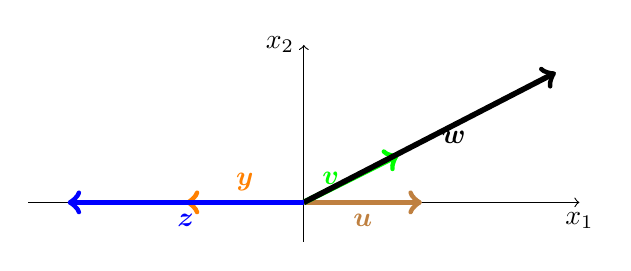
\begin{tikzpicture}
		\begin{scope}[on background layer]
			\onslide<1->{
				\draw[->] (-3.5,0)--(3.5,0) node[below]{$x_1$};
				\draw[->] (0,-0.5)--(0,2) node[left]{$x_2$};
			}
		\end{scope}
		
		\onslide<1->{
			\draw[->, line width=2pt, brown] (0,0)--(1.5,0) node[midway, below]{$\bm{u}$};
			\draw[->, line width=2pt, green] (0,0)--(1.2,0.6) node[midway, left]{$\bm{v}$};
		}
		\onslide<2->{
			\draw[->, line width=2pt, black] (0,0)--(3.2,1.65) node[midway, right]{$\bm{w}$};
		}
		\onslide<3->{
			\draw[->, line width=2pt, orange] (0,0)--(-1.5,0) node[midway, above]{$\bm{y}$};
		}
		\onslide<4->{
			\draw[->, line width=2pt, blue] (0,0)--(-3,0) node[midway, below]{$\bm{z}$};
		}
	\end{tikzpicture}
	
	$$
	\onslide<2->{\bm{u} \cdot \bm{w} >}
	\onslide<1->{\bm{u} \cdot \bm{v} > 0}
	\onslide<3->{> \bm{u} \cdot \bm{y}}
	\onslide<4->{ > \bm{u} \cdot \bm{z}}
	$$
	\onslide<5->{
		Isn't it somehow related to Euclidean distance?
	}
\end{frame}

\begin{frame}{Dot product vs.\ Euclidean distance $\norm{\bm{u} - \bm{v}}_{2} = \sqrt{\sum_{i = 1}^{n} \left( \bm{u}_{[i]} - \bm{v}_{[i]} \right)^2}$}
Let's take the \emph{square} of the Euclidean distance
	$$
	\begin{aligned}
		\left(\norm{\bm{u} - \bm{v}}_{2}\right)^2 &=
		\sum_{i = 1}^{n} \left( \bm{u}_{[i]} - \bm{v}_{[i]} \right)^2 
		=
		\sum_{i = 1}^{n} \left( \bm{u}_{[i]} - \bm{v}_{[i]} \right) \left( \bm{u}_{[i]} - \bm{v}_{[i]} \right) \\ \pause
		&=
		\sum_{i = 1}^{n} \left( \bm{u}_{[i]} \bm{u}_{[i]} + \bm{v}_{[i]} \bm{v}_{[i]} - 2 \bm{u}_{[i]} \bm{v}_{[i]} \right)  \\ \pause
		&= \sum_{i = 1}^{n}  \bm{u}_{[i]} \bm{u}_{[i]} + \sum_{i = 1}^{n} \bm{v}_{[i]} \bm{v}_{[i]} - 2 \sum_{i = 1}^{n} \bm{u}_{[i]} \bm{v}_{[i]} \\
		&= \bm{u} \cdot \bm{u} + \bm{v} \cdot \bm{v} - 2 \bm{u} \cdot \bm{v} \qquad
		\text{( } = 2 - 2 \bm{u} \cdot \bm{v} \text{ for unit vectors)}\\
	\end{aligned}
	$$
	
	\pause
	
$\to$ Minimizing (square) euclidean distance is \emph{proportional} to maximizing cosine similarity (equivalent for unit vectors)

\begin{tikzpicture}[overlay, remember picture] 
	\node at (current page.north east)[anchor = north east, text width=4cm, yshift=-1.3cm] {\scriptsize Conceptual difference: if the origin shifts, the dot product changes, but the distances remains the same \par};
\end{tikzpicture}	
	
	
\end{frame}


\section{Distributional hypothesis}

\begin{frame}{Recall: One-hot encoding of words}
	
Major drawbacks?

\begin{itemize}
	\item No `semantic' similarity, all words are equally `similar'
\end{itemize}

\begin{block}{Example (see Lecture 3 for more)}
	$
	V = \begin{pmatrix}
		\text{a}_1 & \text{abandon}_2 & \ldots & \text{zone}_{2,999} & \text{zoo}_{3,000}
	\end{pmatrix}
	$
	
	\bigskip
	$
	\begin{aligned}
		\text{nice} &= 
		\begin{pmatrix}
			0_1 & \ldots & 1_{1,852} & \ldots & 0_{2,999} & 0_{3,000}
		\end{pmatrix} \\
		\text{pleasant} &= 
		\begin{pmatrix}
			0_1 & \ldots & 1_{2,012} & \ldots & 0_{2,999} & 0_{3,000}
		\end{pmatrix} \\
		\text{horrible} &= 
		\begin{pmatrix}
			0_1 & \ldots & 1_{696} & \ldots & 0_{2,999} & 0_{3,000}
		\end{pmatrix} \\
	\end{aligned}
	$
	
\end{block}


\end{frame}

\begin{frame}{Distributional hypothesis}

The distributional hypothesis stating that \emph{words are similar if they appear in similar contexts}

\begin{example}
Intuitively, when we encounter a sentence with an unknown word such as the word \textbf{wampinuk} in

\pause
\emph{Marco saw a hairy little \textbf{wampinuk} crouching behind a tree}

We infer the meaning of the word based on the context in which it occurs
\end{example}

\end{frame}


\section{From neural LMs to training word embeddings}

\begin{frame}{From neural language models to training word embeddings}
(Neural) language model's goal: Predict probability distribution over $|V|$ for the next word conditioned on the previous words

\begin{itemize}
	\item Side product: Can learn useful word embeddings
\end{itemize}

\pause
What if we don't need probability distribution but just want to learn word embeddings?
\begin{itemize}
	\item We can relax our Markov assumption of `look at $k$ previous words only'
	\item We can get rid of the costly normalization in softmax
\end{itemize}
	
\end{frame}

\begin{frame}{Simplification 1: Ditch the Markov property --- look into the future!}
	\vspace{-1em}
%	$$	f(\bm{x}) = g \left(	\bm{x} \bm{W^1} + \bm{b^1}	\right)	\bm{W^2} + \bm{b^2}	$$
\begin{figure}
	\begin{tikzpicture}	
		%\node (a1) [draw, circle, inner sep=0pt, minimum width=0.75cm, fill=green!20] {$a_1$};
		
		\node (the) [constant] {the};
		\node (black) [constant, below of=the, yshift=-0.5cm, opacity=0.2]{black};
		\node (dog) [constant, below of=black, yshift=-0.5cm]{dog};
		\node (e) [param, below of=dog, yshift=-0.1cm] {$\bm{E}$};
		
		\node (lookup1) [neuron, right of=the, xshift=0.7cm] {$v$};
%		\node (lookup2) [neuron, below of=lookup1, yshift=-0.5cm] {$v$};
		\node (lookup3) [neuron, below of=lookup2, yshift=-0.5cm] {$v$};			
		\node (concat) [neuron, right of=lookup1, xshift=0.5cm, yshift=-1cm] {concat};
		
		
		%			\node (x) [constant, right of=concat, xshift=1cm] {$\bm{x}$};
		\node (f1) [param, right of=concat, xshift=1.5cm] {Lin$(\bm{W^1};\bm{b^1})$};
		
		\node (g) [neuron, right of=f1, xshift=1cm] {$g$};
		\node (f2) [param, right of=g, xshift=1cm] {Lin$(\bm{W^2};\bm{b^2})$};
		
		\node (softmax) [neuron, right of=f2, xshift=1.5cm] {$\softmax$};
		
		\node (l) [neuron, right of=softmax, xshift=1cm] {$L$};
		\node (y) [constant, below of=f2, xshift=1.5cm] {$\bm{y} =$ black};
		
		\begin{scope}[thick, black, ->, >=latex]
			\draw (the) -- (lookup1);
%			\draw (black) -- (lookup2);
			\draw (dog) -- (lookup3);
			\draw (e) -- (lookup1);
%			\draw (e) -- (lookup2);
			\draw (e) -- (lookup3);
			
			\draw (lookup1) -- (concat);
%			\draw (lookup2) -- (concat);
			\draw (lookup3) -- (concat);								
			
			\draw (concat) -- (f1) node [midway, above] {$\bm{x}$};
			\draw (f1) -- (g);
			\draw (g) -- (f2);
			\draw (f2) -- (softmax);
			\draw (softmax) -- (l);
			\draw (y) -- (l);
		\end{scope}	
	\end{tikzpicture}
\end{figure}	

For example, instead of modeling $\Pr(w_3 | w_1, w_2, \boxdot)$, we model $\Pr(w_2 | w_1,  \boxdot, w_3)$

\end{frame}

\begin{frame}{Simplification 2: Give up the costly probability distribution}

Instead of predicting probability distribution over the entire vocabulary, we just want to predict some score of \textbf{context} and \textbf{target word}

What could such a score be?

\pause

\begin{itemize}
	\item Prefer words in their true contexts (high score)
	\pause
	\item Penalize words in their `untrue' contexts (low score)
\end{itemize}

\end{frame}


\begin{frame}{Negative sampling}
	
Instead of predicting probability distribution for the target word, we \textbf{create an artificial binary task} by choosing either the correct or a random incorrect target word \pause
$$
y = 
 \begin{cases}
	1  & \quad \text{if } (w, c_{1:k}) \text{ is a positive example from the corpus}\\
	0  & \quad \text{if } (w', c_{1:k}) \text{ is a negative example from the corpus}\\
\end{cases}
$$

\pause
Which distribution for sampling $w'$ from $V$?
\begin{itemize}
	\item Corpus-based frequency: $\frac{\#(v)}{\sum_{v' \in V} \#(v')}$ (pr.\ of each word $v$)
	\item Re-weighted: $\frac{\#(v)^{0.75}}{\sum_{v' \in V} \#(v')^{0.75}}$ (more weight on less frequent words done in word2vec)
\end{itemize}
	
\end{frame}

\begin{frame}{Turn the problem into binary classification (positive example)}


\begin{figure}
	\begin{tikzpicture}	
		%\node (a1) [draw, circle, inner sep=0pt, minimum width=0.75cm, fill=green!20] {$a_1$};
		
		\node (the) [constant] {the};
		
		\node (black) [constant, below of=the, yshift=-0.5cm, opacity=0.5]{black};

		\node (dog) [constant, below of=black, yshift=-0.5cm]{dog};
		\node (e) [param, below of=dog, yshift=-0.1cm] {$\bm{E}$};
		
		\node (lookup1) [neuron, right of=the, xshift=0.7cm] {$v$};
		\node (lookup2) [neuron, below of=lookup1, yshift=-0.5cm] {$v$};
		\node (lookup3) [neuron, below of=lookup2, yshift=-0.5cm] {$v$};			
		\node (concat) [neuron, right of=lookup1, xshift=1cm, yshift=-1cm] {model the context};
		
		
		%			\node (x) [constant, right of=concat, xshift=1cm] {$\bm{x}$};
		\node (f1) [neuron, right of=concat, xshift=1.5cm, yshift=-1cm] {somehow combine};
		
%		\node (g) [neuron, right of=f1, xshift=1cm] {$g$};
		\node (f2) [param, right of=g, xshift=0cm, yshift=1cm] {some hidden layers};
		
		\node (softmax) [neuron, right of=f2, xshift=1.5cm, yshift=-1cm] {$\sigma$};
		
		\node (l) [neuron, right of=softmax, xshift=1cm] {$L$};
		\node (y) [constant, below of=softmax, xshift=1.5cm] {$y = 1$};
		
		\begin{scope}[thick, black, ->, >=latex]
			\draw (the) -- (lookup1);
			\draw (black) -- (lookup2);
			\draw (dog) -- (lookup3);
			\draw (e) -- (lookup1);
			\draw (e) -- (lookup2);
			\draw (e) -- (lookup3);
			
			\draw (lookup1) -- (concat);
			\draw (lookup2) -- (f1);
			\draw (lookup3) -- (concat);								
			
			\draw (concat) -- (f1);
%			\draw (f1) -- (g);
			\draw (f1) -- (f2);
			\draw (f2) -- (softmax);
			\draw (softmax) -- (l);
			\draw (y) -- (l);
		\end{scope}	
	\end{tikzpicture}
\end{figure}	
	
\end{frame}

\begin{frame}{Turn the problem into binary classification (negative example)}
	
	
	\begin{figure}
		\begin{tikzpicture}	
			%\node (a1) [draw, circle, inner sep=0pt, minimum width=0.75cm, fill=green!20] {$a_1$};
			
			\node (the) [constant] {the};
			
			\node (black) [constant, below of=the, yshift=-0.5cm, opacity=0.5]{with};
			
			\node (dog) [constant, below of=black, yshift=-0.5cm]{dog};
			\node (e) [param, below of=dog, yshift=-0.1cm] {$\bm{E}$};
			
			\node (lookup1) [neuron, right of=the, xshift=0.7cm] {$v$};
			\node (lookup2) [neuron, below of=lookup1, yshift=-0.5cm] {$v$};
			\node (lookup3) [neuron, below of=lookup2, yshift=-0.5cm] {$v$};			
			\node (concat) [neuron, right of=lookup1, xshift=1cm, yshift=-1cm] {model the context};
			
			
			%			\node (x) [constant, right of=concat, xshift=1cm] {$\bm{x}$};
			\node (f1) [neuron, right of=concat, xshift=1.5cm, yshift=-1cm] {somehow combine};
			
			%		\node (g) [neuron, right of=f1, xshift=1cm] {$g$};
			\node (f2) [param, right of=g, xshift=0cm, yshift=1cm] {some hidden layers};
			
			\node (softmax) [neuron, right of=f2, xshift=1.5cm, yshift=-1cm] {$\sigma$};
			
			\node (l) [neuron, right of=softmax, xshift=1cm] {$L$};
			\node (y) [constant, below of=softmax, xshift=1.5cm] {$y = 0$};
			
			\begin{scope}[thick, black, ->, >=latex]
				\draw (the) -- (lookup1);
				\draw (black) -- (lookup2);
				\draw (dog) -- (lookup3);
				\draw (e) -- (lookup1);
				\draw (e) -- (lookup2);
				\draw (e) -- (lookup3);
				
				\draw (lookup1) -- (concat);
				\draw (lookup2) -- (f1);
				\draw (lookup3) -- (concat);								
				
				\draw (concat) -- (f1);
				%			\draw (f1) -- (g);
				\draw (f1) -- (f2);
				\draw (f2) -- (softmax);
				\draw (softmax) -- (l);
				\draw (y) -- (l);
			\end{scope}	
		\end{tikzpicture}
	\end{figure}	
	
\end{frame}



\section{word2vec}

\begin{frame}{word2vec}
word2vec simplifies the neural LM by removing the hidden layer (so turning it into a log-linear model!)

\begin{figure}
	\begin{tikzpicture}	
		%\node (a1) [draw, circle, inner sep=0pt, minimum width=0.75cm, fill=green!20] {$a_1$};
		
		\node (the) [constant] {the};
		
		\node (black) [constant, below of=the, yshift=-0.5cm, opacity=0.5]{black};
		
		\node (dog) [constant, below of=black, yshift=-0.5cm]{dog};
		\node (e) [param, below of=dog, yshift=-0.1cm] {$\bm{E}$};
		
		\node (lookup1) [neuron, right of=the, xshift=0.7cm] {$v$};
		\node (lookup2) [neuron, below of=lookup1, yshift=-0.5cm] {$v$};
		\node (lookup3) [neuron, below of=lookup2, yshift=-0.5cm] {$v$};			
		\node (concat) [neuron, right of=lookup1, xshift=1cm, yshift=-1cm] {model the context};
		
		
		%			\node (x) [constant, right of=concat, xshift=1cm] {$\bm{x}$};
		\node (f1) [neuron, right of=concat, xshift=1.5cm, yshift=-1cm] {somehow combine};
		
		%		\node (g) [neuron, right of=f1, xshift=1cm] {$g$};
		\node (f2) [param, right of=g, xshift=0cm, yshift=1cm] {\sout{some hidden layers}};
		
		\node (softmax) [neuron, right of=f2, xshift=1.5cm, yshift=-1cm] {$\sigma$};
		
		\node (l) [neuron, right of=softmax, xshift=1cm] {$L$};
		\node (y) [constant, below of=softmax, xshift=1.5cm] {$y = 1$};
		
		\begin{scope}[thick, black, ->, >=latex]
			\draw (the) -- (lookup1);
			\draw (black) -- (lookup2);
			\draw (dog) -- (lookup3);
			\draw (e) -- (lookup1);
			\draw (e) -- (lookup2);
			\draw (e) -- (lookup3);
			
			\draw (lookup1) -- (concat);
			\draw (lookup2) -- (f1);
			\draw (lookup3) -- (concat);								
			
			\draw (concat) -- (f1);
			%			\draw (f1) -- (g);
%			\draw (f1) -- (f2);
			\draw (f1) -- (softmax);
			\draw (softmax) -- (l);
			\draw (y) -- (l);
		\end{scope}	
	\end{tikzpicture}
\end{figure}	

\end{frame}


\begin{frame}{word2vec --- how to model the context?}
	
\pause

\begin{figure}
	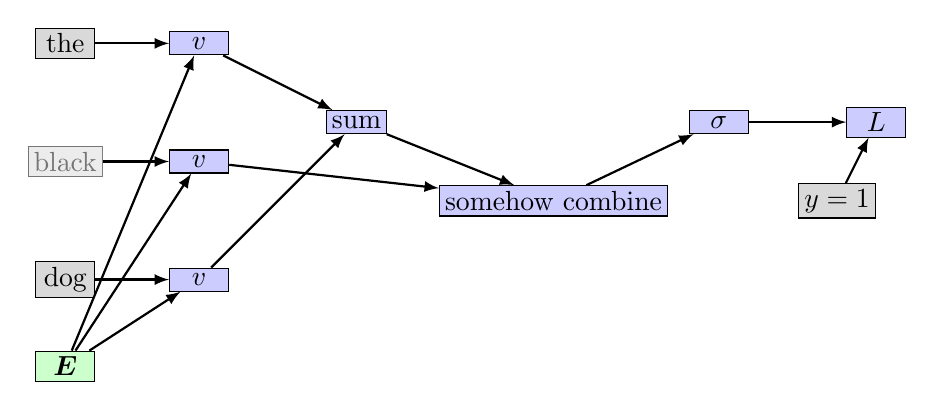
\begin{tikzpicture}	
		%\node (a1) [draw, circle, inner sep=0pt, minimum width=0.75cm, fill=green!20] {$a_1$};
		
		\node (the) [constant] {the};
		
		\node (black) [constant, below of=the, yshift=-0.5cm, opacity=0.5]{black};
		
		\node (dog) [constant, below of=black, yshift=-0.5cm]{dog};
		\node (e) [param, below of=dog, yshift=-0.1cm] {$\bm{E}$};
		
		\node (lookup1) [neuron, right of=the, xshift=0.7cm] {$v$};
		\node (lookup2) [neuron, below of=lookup1, yshift=-0.5cm] {$v$};
		\node (lookup3) [neuron, below of=lookup2, yshift=-0.5cm] {$v$};			
		\node (concat) [neuron, right of=lookup1, xshift=1cm, yshift=-1cm] {sum};
		
		
		%			\node (x) [constant, right of=concat, xshift=1cm] {$\bm{x}$};
		\node (f1) [neuron, right of=concat, xshift=1.5cm, yshift=-1cm] {somehow combine};
		
		%		\node (g) [neuron, right of=f1, xshift=1cm] {$g$};
%		\node (f2) [param, right of=g, xshift=0cm, yshift=1cm] {\sout{something complicated}};
		
		\node (softmax) [neuron, right of=f1, xshift=1.1cm, yshift=1cm] {$\sigma$};
		
		\node (l) [neuron, right of=softmax, xshift=1cm] {$L$};
		\node (y) [constant, below of=softmax, xshift=1.5cm] {$y = 1$};
		
		\begin{scope}[thick, black, ->, >=latex]
			\draw (the) -- (lookup1);
			\draw (black) -- (lookup2);
			\draw (dog) -- (lookup3);
			\draw (e) -- (lookup1);
			\draw (e) -- (lookup2);
			\draw (e) -- (lookup3);
			
			\draw (lookup1) -- (concat);
			\draw (lookup2) -- (f1);
			\draw (lookup3) -- (concat);								
			
			\draw (concat) -- (f1);
			%			\draw (f1) -- (g);
			%			\draw (f1) -- (f2);
			\draw (f1) -- (softmax);
			\draw (softmax) -- (l);
			\draw (y) -- (l);
		\end{scope}	
	\end{tikzpicture}
\end{figure}


%- we have obtained the best performance on the task introduced in the next section by building a log-linear classifier with four future and four history words at the input, where the training criterion is to correctly classify the current (middle) word.

Variant 1: Continuous bag of words (CBOW)
$\bm{c} = \sum_{i = 1}^{k} v(c_i)$


\begin{tikzpicture}[overlay, remember picture] 
	\node at (current page.north east)[ref] {\fullcite{Mikolov.et.al.2013.ICLR} \par};
\end{tikzpicture}


\end{frame}


\begin{frame}{Final CBOW word2vec --- similarity score is the dot product}

%	\vspace{-1em}
	%	$$	f(\bm{x}) = g \left(	\bm{x} \bm{W^1} + \bm{b^1}	\right)	\bm{W^2} + \bm{b^2}	$$
	\begin{figure}
		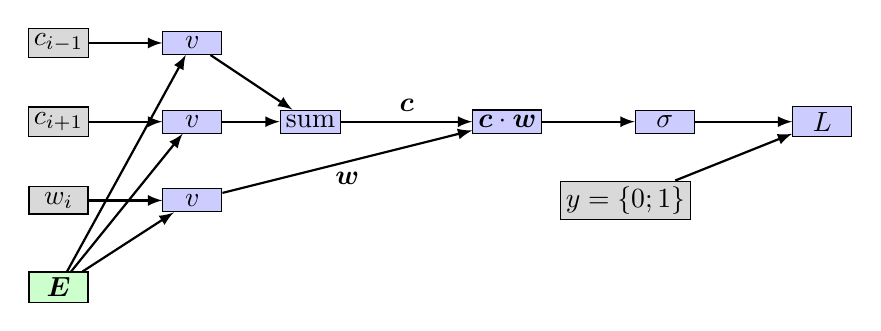
\begin{tikzpicture}	
			%\node (a1) [draw, circle, inner sep=0pt, minimum width=0.75cm, fill=green!20] {$a_1$};
			
			\node (the) [constant] {$c_{i-1}$};
			\node (black) [constant, below of=the, yshift=0cm]{$c_{i+1}$};
			\node (dog) [constant, below of=black, yshift=0cm]{$w_i$};
			\node (e) [param, below of=dog, yshift=-0.1cm] {$\bm{E}$};
			
			\node (lookup1) [neuron, right of=the, xshift=0.7cm] {$v$};
			\node (lookup2) [neuron, below of=lookup1, yshift=0cm] {$v$};
			\node (lookup3) [neuron, below of=lookup2, yshift=0cm] {$v$};			
			\node (concat) [neuron, right of=lookup1, xshift=0.5cm, yshift=-1cm] {sum};
			
			
			%			\node (x) [constant, right of=concat, xshift=1cm] {$\bm{x}$};
			\node (f1) [neuron, right of=concat, xshift=1.5cm] {$\bm{c} \cdot \bm{w}$};
			
			\node (sigma) [neuron, right of=f1, xshift=1cm] {$\sigma$};
			
			\node (l) [neuron, right of=sigma, xshift=1cm] {$L$};
			\node (y) [constant, below of=f1, xshift=1.5cm] {$y = \{0; 1\}$};
			
			\begin{scope}[thick, black, ->, >=latex]
				\draw (the) -- (lookup1);
				\draw (black) -- (lookup2);
				\draw (dog) -- (lookup3);
				\draw (e) -- (lookup1);
				\draw (e) -- (lookup2);
				\draw (e) -- (lookup3);
				
				\draw (lookup1) -- (concat);
				\draw (lookup2) -- (concat);
				\draw (lookup3) -- (f1) node [midway, below] {$\bm{w}$};
				
				\draw (concat) -- (f1) node [midway, above] {$\bm{c}$};
				\draw (f1) -- (sigma);
				\draw (sigma) -- (l);
				\draw (y) -- (l);
			\end{scope}	
		\end{tikzpicture}
	\end{figure}	

\vspace{-1em}
	$w_i$ --- target word, $c_{i-1}, c_{i+1}$ --- context words (one-hot)
	
	$y = 1$ for correct word-context pairs, $y = 0$ for random $w_i$
	
	The only learnable parameter is the embedding matrix $\bm{E}$
	
	What is $\sigma(\bm{c} \cdot \bm{w})$ doing?
	
\end{frame}

\begin{frame}{word2vec: Learning useful word embeddings}
	
Train the network to distinguish `good' word-context pairs from `bad' ones

Create a set $D$ of correct word-context pairs and set $\bar{D}$ of incorrect word-context pairs

The goal of the algorithm is to estimate the probability $\Pr(D = 1 \mid w, c)$ that the word-context pair $w, c$ comes from the correct set $D$

This should be high ($\to 1$) for pairs from $D$ and low ($\to 0$) for pairs from $\bar{D}$
\end{frame}



\section{Advantages and limitations of words embeddings}

\begin{frame}{Using word embeddings}

Pre-trained embeddings: `Semantic' input to any neural network instead of one-hot word encoding
\begin{itemize}
	\item Instance of \textbf{transfer learning} --- pre-trained (self-trained) on an auxiliary task, plugged into a more complex model as pre-trained weights
\end{itemize}

Example: Represent a document as an average of its words' embeddings (average bag-of-words through embeddings) for text classification

\bigskip

Side note: word2vec and word embeddings $\to$ part of the deep-learning revolution in NLP around 2015

\end{frame}

\begin{frame}{Semantic similarity, short document similarity, query expansion}

\onslide<1->{
\emph{``Using Word2Vec's CBOW embedding approach, applied over the entire corpus on which search is performed, we select terms that are semantically related to the query."}

\bigskip
}

\onslide<2->{
What can possibly go wrong?
}

\onslide<1->{
\begin{tikzpicture}[overlay, remember picture] 
	\node at (current page.north east)[ref] {\fullcite{Kuzi.et.al.2016.CIKM} \par};
\end{tikzpicture}
}
\end{frame}

\begin{frame}
	
\begin{figure}
	\includegraphics[trim={0 6cm 0 0},clip,width=0.80\linewidth]{img/rewe.png}
\end{figure}


\begin{tikzpicture}[overlay, remember picture] 
\node at (current page.north east)[anchor = north east, text width=4cm, yshift=-1.3cm] {\scriptsize 

Searched for \textbf{covid} (test), returned the closest items with \textbf{corona} in the title (because their embeddings learned that covid $\approx$ corona). \\ \bigskip

Query expansion with word embeddings might be tricky \par};
\end{tikzpicture}
\end{frame}

\begin{frame}{Mining word analogies with word2vec}

\begin{block}{`Germany to Berlin is France to ?'}
Solved by $v(\text{Berlin}) - v(\text{Germany}) + v(\text{France})$, outputs vector $\bm{x}$ which is closest to Paris in the embeddings space (the closest row in $\bm{E}$)
\end{block}

\begin{block}{Find the queen}
$v(\text{king}) - v(\text{man}) + v(\text{woman}) \approx v(\text{queen})$
\end{block}


\end{frame}

\begin{frame}{Limitations of word embeddings (1)}

\begin{block}{Definition of similarity}
Completely operational: words are similar if used in similar contexts
\end{block}

\begin{block}{Antonyms}
Words opposite of each other (buy---sell, hot---cold) tend to appear in similar contexts (things that can be hot can also be cold, things that are bought are often sold)

Models might tend to judge antonyms as very similar to each other
\end{block}

\end{frame}

\begin{frame}{Limitations of word embeddings (2)}

\begin{block}{Biases}
Distributional methods reflect the usage patterns in the corpora on which they are based

The corpora reflect human biases in the real world (cultural or otherwise)
	
\emph{``Word embeddings encode not only stereotyped biases but also other knowledge
[..] are problematic as toward race or gender, or even simply veridical, reflecting the status quo distribution of gender with respect to careers or first names.''}
\end{block}


\begin{tikzpicture}[overlay, remember picture] 
	\node at (current page.north east)[ref] {\fullcite{Caliskan.et.al.2017.science} \par};
\end{tikzpicture}

\end{frame}

\begin{frame}{Limitations of word embeddings (3)}
	
\begin{block}{Polysemy, context independent representation}
Some words have obvious multiple senses

A \emph{bank} may refer to a financial institution or to the side of a river, a \emph{star} may be an abstract shape, a celebrity, an astronomical entity

Using a single vector for all forms	is problematic
\end{block}


\end{frame}


\section*{Recap}



\begin{frame}{Take aways}
	
\begin{itemize}
	\item Self-supervised training of word embeddings
	\item word2vec trained with negative sampling
	\item CBOW and skip-gram for context modeling
\end{itemize}
	
\end{frame}



\begin{frame}{License and credits}

	\begin{columns}
		\begin{column}{0.7\textwidth}
			Licensed under Creative Commons Attribution-ShareAlike 4.0 International (CC BY-SA 4.0)
		\end{column}
		\begin{column}{0.2\textwidth}
			\includegraphics[width=0.9\linewidth]{img/cc-by-sa-icon.pdf}
		\end{column}
	\end{columns}
	
	\bigskip
	
	Credits
	
	\begin{scriptsize}
		
		Ivan Habernal
		
		Content from ACL Anthology papers licensed under CC-BY \url{https://www.aclweb.org/anthology}
		
	
	\end{scriptsize}
	
\end{frame}


\appendix

\section*{Skip-Gram in word2vec}

\begin{frame}{Skip-Gram --- even more relaxed context notion}

\begin{figure}
	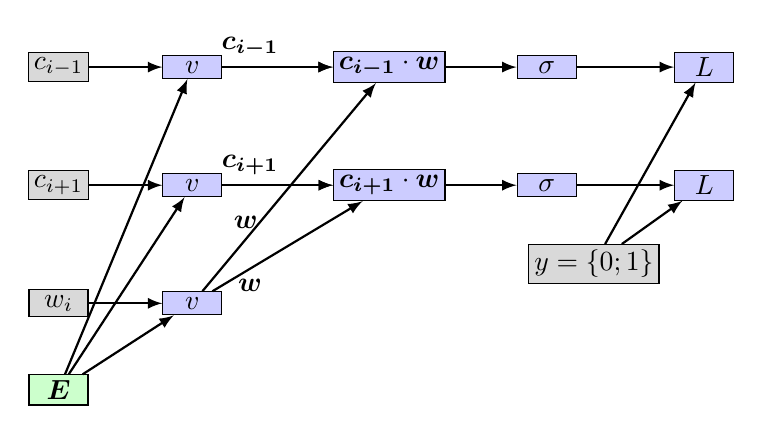
\begin{tikzpicture}	
		%\node (a1) [draw, circle, inner sep=0pt, minimum width=0.75cm, fill=green!20] {$a_1$};
		
		\node (the) [constant] {$c_{i-1}$};
		\node (black) [constant, below of=the, yshift=-0.5cm]{$c_{i+1}$};
		\node (dog) [constant, below of=black, yshift=-0.5cm]{$w_i$};
		\node (e) [param, below of=dog, yshift=-0.1cm] {$\bm{E}$};
		
		\node (lookup1) [neuron, right of=the, xshift=0.7cm] {$v$};
		\node (lookup2) [neuron, below of=lookup1, yshift=-0.5cm] {$v$};
		\node (lookup3) [neuron, below of=lookup2, yshift=-0.5cm] {$v$};			
%		\node (concat) [neuron, right of=lookup1, xshift=0.5cm, yshift=-1cm] {sum};
		
		
		%			\node (x) [constant, right of=concat, xshift=1cm] {$\bm{x}$};
		\node (f11) [neuron, right of=lookup1, xshift=1.5cm] {$\bm{c_{i-1}} \cdot \bm{w}$};
		\node (f12) [neuron, right of=lookup2, xshift=1.5cm] {$\bm{c_{i+1}} \cdot \bm{w}$};
		
		\node (sigma1) [neuron, right of=f11, xshift=1cm] {$\sigma$};
		\node (sigma2) [neuron, right of=f12, xshift=1cm] {$\sigma$};
		
		\node (l1) [neuron, right of=sigma1, xshift=1cm] {$L$};
		\node (l2) [neuron, right of=sigma2, xshift=1cm] {$L$};
		\node (y) [constant, below of=sigma2, xshift=0.6cm] {$y = \{0; 1\}$};
		
		\begin{scope}[thick, black, ->, >=latex]
			\draw (the) -- (lookup1);
			\draw (black) -- (lookup2);
			\draw (dog) -- (lookup3);
			\draw (e) -- (lookup1);
			\draw (e) -- (lookup2);
			\draw (e) -- (lookup3);
			
			\draw (lookup1) -- (f11);
			\draw (lookup2) -- (f12);
			\draw (lookup3) -- (f11) node [near start, above] {$\bm{w}$};
			\draw (lookup3) -- (f12) node [near start, below] {$\bm{w}$};			
			
			\draw (lookup1) -- (f11) node [near start, above] {$\bm{c_{i-1}}$};
			\draw (lookup2) -- (f12) node [near start, above] {$\bm{c_{i+1}}$};
			\draw (f11) -- (sigma1);
			\draw (f12) -- (sigma2);
			\draw (sigma1) -- (l1);
			\draw (sigma2) -- (l2);
			\draw (y) -- (l1);
			\draw (y) -- (l2);
		\end{scope}	
	\end{tikzpicture}
\end{figure}

For $k$-element context $c_{1:k}$, treat as $k$ different independent contexts $(w_i, c_i)$


\end{frame}

\begin{frame}{Choosing the context}

\begin{block}{Sliding window approach --- CBOW}
Auxiliary tasks are created by taking a sequence of $2m + 1$ words
\begin{itemize}
	\item The middle word is the target (focus) word
	\item The $m$ words to each side is the context
\end{itemize}
\end{block}

\begin{block}{Sliding window approach --- Skip-Gram}
$2m$ distinct tasks are created, each pairing the focus word with a different context word
\end{block}	

Skip-gram-based approaches shown to be robust and efficient to train

\end{frame}

\section*{FastText embeddings: Sub-word embeddings}

\begin{frame}{FastText embeddings}

Popular word embedding models ignore the morphology of words, by assigning a distinct vector to each word.
\begin{itemize}
\item Limitation, especially for languages with large vocabularies and many rare words
\end{itemize}

\pause

$\to$ Model each word as a bag of character $n$-grams
\begin{itemize}
\item Each character $n$-gram has own embedding
\item Word is represented as a sum of $n$-gram embeddings	
\end{itemize}

\begin{tikzpicture}[overlay, remember picture] 
	\node at (current page.north east)[ref] {\fullcite{Bojanowski.et.al.2017.TACL} \par};
\end{tikzpicture}


\end{frame}

\begin{frame}{FastText embeddings example}
	
Extract all the character $n$-grams for $3 \leq n \leq 6$

\begin{example}
\texttt{eating} $\to$ $G_w = \{$
\texttt{<ea}, \texttt{eat}, \texttt{ati}, \texttt{tin}, \texttt{ing}, \texttt{ng>},
\texttt{<eat}, \texttt{eati}, \texttt{atin}, \texttt{ting}, \texttt{ing>},
\texttt{<eati}, \texttt{eatin}, \texttt{ating}, \texttt{ting>},
\texttt{<eatin}, \texttt{eating}, \texttt{ating>} $\}$
$$
v(\text{eating}) = \sum_{g \in G_w} v(G_w)
$$
\end{example}

Train with skip-gram and negative sampling (same as word2vec)

\begin{tikzpicture}[overlay, remember picture] 
	\node at (current page.north east)[ref] {\fullcite{Bojanowski.et.al.2017.TACL} \par};
\end{tikzpicture}



	
\end{frame}



\end{document}

